% -*- TeX-engine: xetex; eval: (auto-fill-mode 0); eval: (visual-line-mode 1); -*-
% Compile with XeLaTeX

%%%%%%%%%%%%%%%%%%%%%%%
% Option 1: Slides: (comment for handouts)   %
%%%%%%%%%%%%%%%%%%%%%%%
%
%\documentclass[slidestop,compress,mathserif,12pt,t,professionalfonts,xcolor=table]{beamer}
%
%% solution stuff
%\newcommand{\solnMult}[1]{
%\only<1>{#1}
%\only<2->{\red{\textbf{#1}}}
%}
%\newcommand{\soln}[1]{\textit{#1}}

%%%%%%%%%%%%%%%%%%%%%%%%%%%%%%%
% Option 2: Handouts, without solutions (post before class)    %
%%%%%%%%%%%%%%%%%%%%%%%%%%%%%%%

 \documentclass[11pt,containsverbatim,handout,xcolor=xelatex,dvipsnames,table]{beamer}

 % handout layout
 \usepackage{pgfpages}
 \pgfpagesuselayout{4 on 1}[letterpaper,landscape,border shrink=5mm]

 % solution stuff
 \newcommand{\solnMult}[1]{#1}
 \newcommand{\soln}[1]{}

%%%%%%%%%%%%%%%%%%%%%%%%%%%%%%%%%%%%
% Option 3: Handouts, with solutions (may post after class if need be)    %
%%%%%%%%%%%%%%%%%%%%%%%%%%%%%%%%%%%%

% \documentclass[11pt,containsverbatim,handout,xcolor=xelatex,dvipsnames,table]{beamer}

% % handout layout
% \usepackage{pgfpages}
% \pgfpagesuselayout{4 on 1}[letterpaper,landscape,border shrink=5mm]

% % solution stuff
% \newcommand{\solnMult}[1]{\red{\textbf{#1}}}
% \newcommand{\soln}[1]{\textit{#1}}

%%%%%%%%%%
% Load style file, defaults  %
%%%%%%%%%%

%%%%%%%%%%%%%%%%
% Themes
%%%%%%%%%%%%%%%%

% See http://deic.uab.es/~iblanes/beamer_gallery/ for mor options

% Style theme
\usetheme{metropolis}

% Color theme
%\usecolortheme{seahorse}

% Helvetica Neue Light for most text
%\usepackage{fontspec}
%\setsansfont{Helvetica Neue Light}

%%%%%%%%%%%%%%%%
% Packages
%%%%%%%%%%%%%%%%

\usepackage{geometry}
\usepackage{graphicx}
\usepackage{amssymb}
\usepackage{epstopdf}
\usepackage{amsmath}  	% this permits text in eqnarray among other benefits
\usepackage{url}		% produces hyperlinks
\usepackage[english]{babel}
\usepackage{colortbl}	% allows for color usage in tables
\usepackage{multirow}	% allows for rows that span multiple rows in tables
\usepackage{color}		% this package has a variety of color options
\usepackage{pgf}
\usepackage{calc}
\usepackage{ulem}
\usepackage{multicol}
\usepackage{textcomp}
\usepackage{listings}
\usepackage{changepage}
\usepackage{tikz}
\usetikzlibrary{trees}		% for probability trees
\usepackage{fancyvrb}	% for colored code chunks
\usepackage{nameref}

%%%%%%%%%%%%%%%%
% Remove navigation symbols
%%%%%%%%%%%%%%%%

\beamertemplatenavigationsymbolsempty
\hypersetup{pdfpagemode=UseNone} % don't show bookmarks on initial view

%%%%%%%%%%%%%%%%
% User defined colors
%%%%%%%%%%%%%%%%

% Pantone 2016 Spring colors
% https://atelierbram.github.io/c-tiles16/colorscheming/pantone-spring-2016-colortable.html
% update each semester or year

\xdefinecolor{custom_blue}{rgb}{0.01, 0.31, 0.52} % Snorkel Blue
\xdefinecolor{custom_darkBlue}{rgb}{0.20, 0.20, 0.39} % Reflecting Pond  
\xdefinecolor{custom_orange}{rgb}{0.96, 0.57, 0.42} % Cadmium Orange
\xdefinecolor{custom_green}{rgb}{0, 0.47, 0.52} % Biscay Bay
\xdefinecolor{custom_red}{rgb}{0.58, 0.32, 0.32} % Marsala

\xdefinecolor{custom_lightGray}{rgb}{0.78, 0.80, 0.80} % Glacier Gray
\xdefinecolor{custom_darkGray}{rgb}{0.35, 0.39, 0.43} % Stormy Weather

%%%%%%%%%%%%%%%%
% Template colors
%%%%%%%%%%%%%%%%

%\setbeamercolor*{palette primary}{fg=white,bg= custom_blue}
%\setbeamercolor*{palette secondary}{fg=black,bg= custom_blue!80!black}
%\setbeamercolor*{palette tertiary}{fg=white,bg= custom_blue!80!black!80}
%\setbeamercolor*{palette quaternary}{fg=white,bg= custom_blue}
%
%\setbeamercolor{structure}{fg= custom_blue}
%\setbeamercolor{frametitle}{bg= custom_blue!90}
%\setbeamertemplate{blocks}[shadow=false]
%\setbeamersize{text margin left=2em,text margin right=2em}

%%%%%%%%%%%%%%%%
% Styling fonts, bullets, etc.
%%%%%%%%%%%%%%%%
%
%% title slide
%\setbeamerfont{title}{size=\large,series=\bfseries}
%\setbeamerfont{subtitle}{size=\large,series=\mdseries}
%%\setbeamerfont{institute}{size=\large,series=\mdseries}
%
% color of alerted text
\setbeamercolor{alerted text}{fg=custom_orange}

% styling of itemize bullets
\setbeamercolor{item}{fg=custom_blue}
\setbeamertemplate{itemize item}{{{\small$\blacktriangleright$}}}
\setbeamercolor{subitem}{fg=custom_blue}
\setbeamertemplate{itemize subitem}{{\textendash}}
\setbeamerfont{itemize/enumerate subbody}{size=\footnotesize}
\setbeamerfont{itemize/enumerate subitem}{size=\footnotesize}

% styling of enumerate bullets
\setbeamertemplate{enumerate item}{\insertenumlabel.}

%\setbeamerfont{enumerate item}{family={\fontspec{Helvetica Neue}}}
%\setbeamerfont{enumerate subitem}{family={\fontspec{Helvetica Neue}}}
%\setbeamerfont{enumerate subsubitem}{family={\fontspec{Helvetica Neue}}}

% make frame titles small to make room in the slide
\setbeamerfont{frametitle}{size=\small} 




%% set Helvetica Neue font for frame and section titles
%\setbeamerfont{frametitle}{family={\fontspec{Helvetica Neue}}}
%\setbeamerfont{sectiontitle}{family={\fontspec{Helvetica Neue}}}
%\setbeamerfont{section in toc}{family={\fontspec{Helvetica Neue}}}
%\setbeamerfont{subsection in toc}{family={\fontspec{Helvetica Neue}}, size=\small}
%\setbeamerfont{footline}{family={\fontspec{Helvetica Neue}}}
%\setbeamerfont{subsection in toc}{family={\fontspec{Helvetica Neue}}}
%\setbeamerfont{block title}{family={\fontspec{Helvetica Neue}}}
%
%%%%%%%%%%%%%%%%%
%% New fonts accessed by fontspec package
%%%%%%%%%%%%%%%%%
%
%% Monaco font for code
%\newfontfamily{\monaco}{Monaco}

%%%%%%%%%%%%%%%%
% Color text commands
%%%%%%%%%%%%%%%%

%orange
\newcommand{\orange}[1]{\textit{\textcolor{custom_orange}{#1}}}

% yellow
\newcommand{\yellow}[1]{\textit{\textcolor{yellow}{#1}}}

% blue
\newcommand{\blue}[1]{\textit{\textcolor{blue}{#1}}}

% green
\newcommand{\green}[1]{\textit{\textcolor{custom_green}{#1}}}

% red
\newcommand{\red}[1]{\textit{\textcolor{custom_red}{#1}}}

% dark gray
\newcommand{\darkgray}[1]{\textit{\textcolor{custom_darkGray}{#1}}}

% light gray
\newcommand{\lightgray}[1]{\textit{\textcolor{custom_lightGray}{#1}}}

% pink
\newcommand{\pink}[1]{\textit{\textcolor{pink}{#1}}}


%%%%%%%%%%%%%%%%
% Custom commands
%%%%%%%%%%%%%%%%

% empty box for probability tree frame
\newcommand{\emptybox}[2]{
	\fbox{ \begin{minipage}{#1} \hfill\vspace{#2} \end{minipage} }
}

% cancel
\newcommand{\cancel}[1]{%
    \tikz[baseline=(tocancel.base)]{
        \node[inner sep=0pt,outer sep=0pt] (tocancel) {#1};
        \draw[red, line width=0.5mm] (tocancel.south west) -- (tocancel.north east);
    }%
}

% degree
\newcommand{\degree}{\ensuremath{^\circ}}

% cite
\newcommand{\ct}[1]{
\vfill
{\tiny #1}}

% Note
\newcommand{\Note}[1]{
\rule{2.5cm}{0.25pt} \\ \textit{\footnotesize{\textcolor{custom_red}{Note:} \textcolor{custom_darkGray}{#1}}}}

% Remember
\newcommand{\Remember}[1]{\textit{\scriptsize{\textcolor{custom_red}{Remember:} #1}}}

% links: webURL, webLink
\newcommand{\webURL}[1]{\urlstyle{same}{\textit{\textcolor{custom_blue}{\url{#1}}}}}
\newcommand{\webLink}[2]{\href{#1}{\textcolor{custom_blue}{{#2}}}}

% mail
\newcommand{\mail}[1]{\href{mailto:#1}{\textit{\textcolor{custom_blue}{#1}}}}

% highlighting: hl, hlGr, mathhl
\newcommand{\hl}[1]{\textit{\textcolor{custom_blue}{#1}}}
\newcommand{\hlGr}[1]{\textit{\textcolor{custom_green}{#1}}}
\newcommand{\mathhl}[1]{\textcolor{custom_blue}{\ensuremath{#1}}}

% example
\newcommand{\ex}[1]{\textcolor{blue}{{{\small (#1)}}}}

% twocol: two columns
\newenvironment{twocol}[4]{
\begin{columns}[c]
\column{#1\textwidth}
#3
\column{#2\textwidth}
#4
\end{columns}
}

% threecol: three columns
\newenvironment{threecol}[6]{
\begin{columns}[c]
\column{#1\textwidth}
#4
\column{#2\textwidth}
#5
\column{#3\textwidth}
#6
\end{columns}
}

% slot (for probability calculations)
\newenvironment{slot}[2]{
\begin{array}{c} 
\underline{#1} \\ 
#2
\end{array}
}

% pr: left and right parentheses
\newcommand{\pr}[1]{
\left( #1 \right)
}

%%%%%%%%%%%%%%%%
% Custom blocks
%%%%%%%%%%%%%%%%

% activity: less commonly used
\newcommand{\activity}[2]{
\setbeamertemplate{itemize item}{{{\small\textcolor{custom_orange}{$\blacktriangleright$}}}}
\setbeamercolor{block title}{fg=white, bg=custom_orange}
\setbeamerfont{block title}{size=\small}
\setbeamercolor{block body}{fg=black, bg=custom_orange!20!white!80}
\setbeamerfont{block body}{size=\small}
\begin{block}{Activity: #1}
\setlength\abovedisplayskip{0pt}
#2
\end{block}
}

% app: application exercise
\newcommand{\app}[2]{
\setbeamercolor{block title}{fg=white,bg=custom_green}
\setbeamercolor{block body}{fg=black,bg=custom_green!20!white!80}
\begin{block}{{\small Application exercise: #1}}
#2
\end{block}
}

% disc: discussion question
\newcommand{\disc}[1]{
\vspace*{-2ex}
\setbeamercolor{block body}{bg=custom_blue!25!white!80, fg=custom_blue!55!black!95}
\begin{block}{\vspace*{-3ex}}
#1
\end{block}
\vspace*{-1ex}
}

% clicker: clicker question
\newcommand{\clicker}[1]{
\setbeamercolor{block title}{bg=custom_blue!80!white!50,fg=custom_blue!30!black!90}
\setbeamercolor{block body}{bg=custom_blue!20!white!80,fg=custom_blue!30!black!90}
\begin{block}{\vspace*{-0.2ex}{\footnotesize Your turn}\vspace*{-0.2ex}}
#1
\end{block}
}

% formula
\newcommand{\formula}[2]{
\setbeamercolor{block title}{bg=custom_blue!40!white!60,fg=custom_blue!55!black!95}
\begin{block}{{\small#1}}
#2
\end{block}
}

% code
\newcommand{\Rcode}[1]{
{\monaco {\footnotesize \textcolor{custom_darkBlue}{#1}}}
}

% output
\newcommand{\Rout}[1]{
{\monaco {\footnotesize \textcolor{custom_darkGray}{#1}}}
}

%%%%%%%%%%%%%%%%
% Change margin
%%%%%%%%%%%%%%%%

\newenvironment{changemargin}[2]{%
\begin{list}{}{%
\setlength{\topsep}{0pt}%
\setlength{\leftmargin}{#1}%
\setlength{\rightmargin}{#2}%
\setlength{\listparindent}{\parindent}%
\setlength{\itemindent}{\parindent}%
\setlength{\parsep}{\parskip}%
}%
\item}{\end{list}}

%%%%%%%%%%%%%%%%
% Footnote
%%%%%%%%%%%%%%%%

\long\def\symbolfootnote[#1]#2{\begingroup%
\def\thefootnote{\fnsymbol{footnote}}\footnote[#1]{#2}\endgroup}

%%%%%%%%%%%%%%%%
% Graphics
%%%%%%%%%%%%%%%%

\DeclareGraphicsRule{.tif}{png}{.png}{`convert #1 `dirname #1`/`basename #1 .tif`.png}

%%%%%%%%%%%%%%%%
% Slide number
%%%%%%%%%%%%%%%%

\setbeamertemplate{footline}{%
    \raisebox{5pt}{\makebox[\paperwidth]{\hfill\makebox[20pt]{\color{gray}
          \scriptsize\insertframenumber}}}\hspace*{5pt}}

          
%%%%%%%%%%%%%%%%
% Remove page numbers
%%%%%%%%%%%%%%%%

\newcommand{\removepagenumbers}{% 
  \setbeamertemplate{footline}{}
}

%%%%%%%%%%%%%%%%
% TOC slides
%%%%%%%%%%%%%%%%

\setbeamertemplate{section in toc}{\inserttocsectionnumber.~\inserttocsection}
\setbeamertemplate{subsection in toc}{$\qquad$\inserttocsubsectionnumber.~\inserttocsubsection \\}

\AtBeginSection[] 
{ 
  \addtocounter{framenumber}{-1} 
  % 
  {\removepagenumbers 
  {\small
    \begin{frame}<beamer> 
    \frametitle{Outline} 
    \tableofcontents[currentsection] 
  \end{frame} 
  } 
  }
} 

\AtBeginSubsection[] 
{ 
  \addtocounter{framenumber}{-1} 
  % 
  {\removepagenumbers 
  {\small
    \begin{frame}<beamer> 
    \frametitle{Outline} 
    \tableofcontents[currentsection,currentsubsection] 
  \end{frame} 
  } 
  }
}
% Course Name
\newcommand{\CourseName}{GOVT 3990 - Spring 2017}
\newcommand{\InstituteName}{Cornell University}

% Personal Info
\newcommand{\FirstName}{Sergio}
\newcommand{\LastName}{Garcia-Rios}

% Electronic Info
\newcommand{\PersonalSite}{https://garciarios.github.io}
\newcommand{\CourseSite}{http://garciarios.github.io/govt_3990/}
\newcommand{\Email}{garcia.rios@cornell.edu}

% Exam Dates
\newcommand{\ExamADate}{Feb 24, Wed}
\newcommand{\ExamBDate}{Mar 30, Wed}
\newcommand{\FinalDate}{May 5, Thu - 7-10pm}
% ALT ALT
% % Course Name
\newcommand{\CourseName}{Sta 101 - Spring 2016}
\newcommand{\InstituteName}{Duke University, Department of Statistical Science}

% Personal Info
\newcommand{\FirstName}{Anthea}
\newcommand{\LastName}{Monod}

% Electronic Info
\newcommand{\PersonalSite}{https://stat.duke.edu/people/anthea-monod.html}
\newcommand{\CourseSite}{https://stat.duke.edu/courses/Spring16/sta101.002}
\newcommand{\Email}{anthea@stat.duke.edu}

% Exam Dates
\newcommand{\ExamADate}{Feb 25, Thu}
\newcommand{\ExamBDate}{Mar 31, Thu}
\newcommand{\FinalDate}{???}

%%%%%%%%%%%
% Cover slide info    %
%%%%%%%%%%%

\title{Unit 3: Foundations for inference}
\subtitle{4. MT 1 Review}
\author{\CourseName}
\date{}
\institute{\InstituteName}


%%%%%%%%%%%%%%%%%%%%%%%%%
% Begin document and set Helvetica Neue font   %
%%%%%%%%%%%%%%%%%%%%%%%%%

\begin{document}
\fontspec[Ligatures=TeX]{Helvetica Neue Light}

%%%%%%%%%%%%%%%%%%%%%%%%%%%%%%%%%%%

% Title Page

\begin{frame}[plain]

\titlepage

\vfill

{\scriptsize \webLink{\PersonalSite}{Dr. \LastName{}} \hfill Slides posted at  \webURL{\CourseSite}}

\addtocounter{framenumber}{-1} 

\end{frame}

%%%%%%%%%%%%%%%%%%%%%%%%%%%%%%%%%%%%

\section{Housekeeping}

%%%%%%%%%%%%%%%%%%%%%%%%%%%%%%%%%%%%

\begin{frame}
\frametitle{Announcements}

\begin{itemize}

\item Discussion section tomorrow: More midterm review

\end{itemize}

\end{frame}

%%%%%%%%%%%%%%%%%%%%%%%%%%%%%%%%%%%%

\section{Review}

%%%%%%%%%%%%%%%%%%%%%%%%%%%%%%%%%%%%

\subsection{CLT}

%%%%%%%%%%%%%%%%%%%%%%%%%%%%%%%%%%%%

\begin{frame}

\disc{{\small A housing survey was conducted to determine the price of a typical home in Topanga, CA. The mean price of a house was roughly \$1.3 million with a standard deviation of \$300,000. There were no houses listed below \$600,000 but a few houses above \$3 million.}}

\clicker{Can we estimate the probability that the mean of 60 randomly chosen houses in Topanga is more than \$1.4 million?}

\begin{enumerate}[(a)]
\item \solnMult{yes}
\item no
\end{enumerate}

\end{frame}

%%%%%%%%%%%%%%%%%%%%%%%%%%%%%%%%%%%%

\begin{frame}

\disc{{\small A housing survey was conducted to determine the price of a typical home in Topanga, CA. The mean price of a house was roughly \$1.3 million with a standard deviation of \$300,000. There were no houses listed below \$600,000 but a few houses above \$3 million.}}

\disc{{\small What is the probability that the mean of 60 randomly chosen houses in Topanga is more than \$1.4 million?}}

\pause

In order to calculate $P(\bar{X} > 1.4~mil)$, we need to first determine the distribution of $\bar{X}$. According to the CLT,

\pause

\[ \bar{X} \pause \sim N \pause \left( mean = 1.3, \pause SE = \frac{0.3}{\sqrt{60}} = 0.0387 \right) \]

\pause

\begin{eqnarray*}
P(\bar{X} > 1.4 ) &=& P\left(Z > \frac{1.4 - 1.3}{0.0387}\right) \\
\pause
&=& P(Z > 2.58) \\
\pause
&=& 1 - 0.9951 \pause =  0.0049
\end{eqnarray*}

\end{frame}

%%%%%%%%%%%%%%%%%%%%%%%%%%%%%%%%%%%%

\subsection{Numerical distributions}

%%%%%%%%%%%%%%%%%%%%%%%%%%%%%%%%%%%%

\begin{frame}

\clicker{Which of the following is \underline{false}?}

\begin{center}
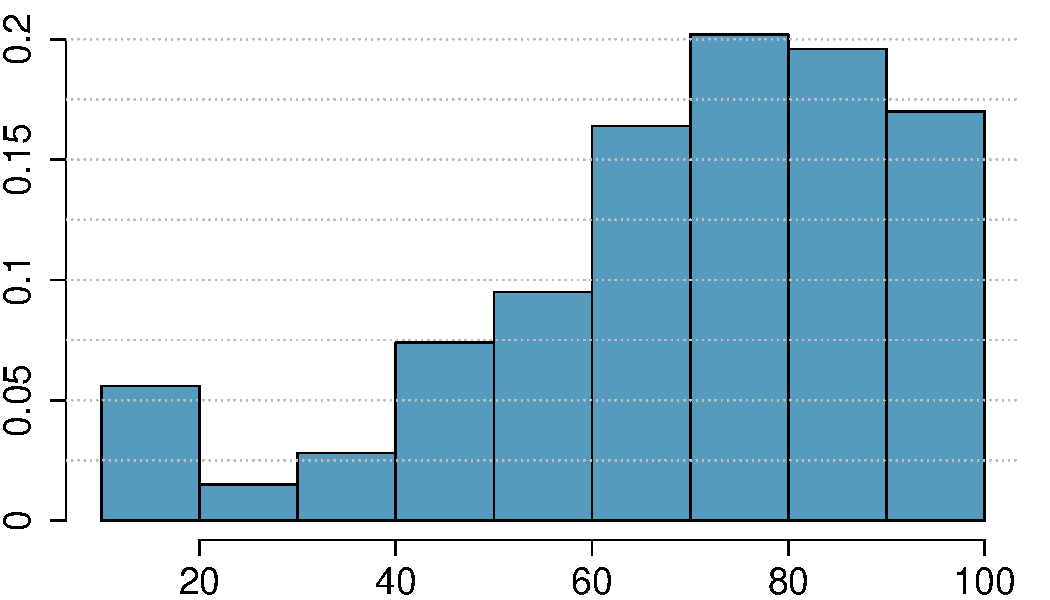
\includegraphics[width=0.55\textwidth]{figures/num_data/rel_hist}
\end{center}

\begin{enumerate}[(a)]
\item The box plot would have outliers only on the lower end.
\item The median is between 70 and 80.
\item \solnMult{More than 25\% of the data is above 90.}
\item More than 50\% of the data have positive Z scores.
\item The mean is likely to be smaller than the median.
\end{enumerate}

\end{frame}

%%%%%%%%%%%%%%%%%%%%%%%%%%%%%%%%%%%%

\begin{frame}

\clicker{Which of the following is not necessarily true?}

\begin{center}
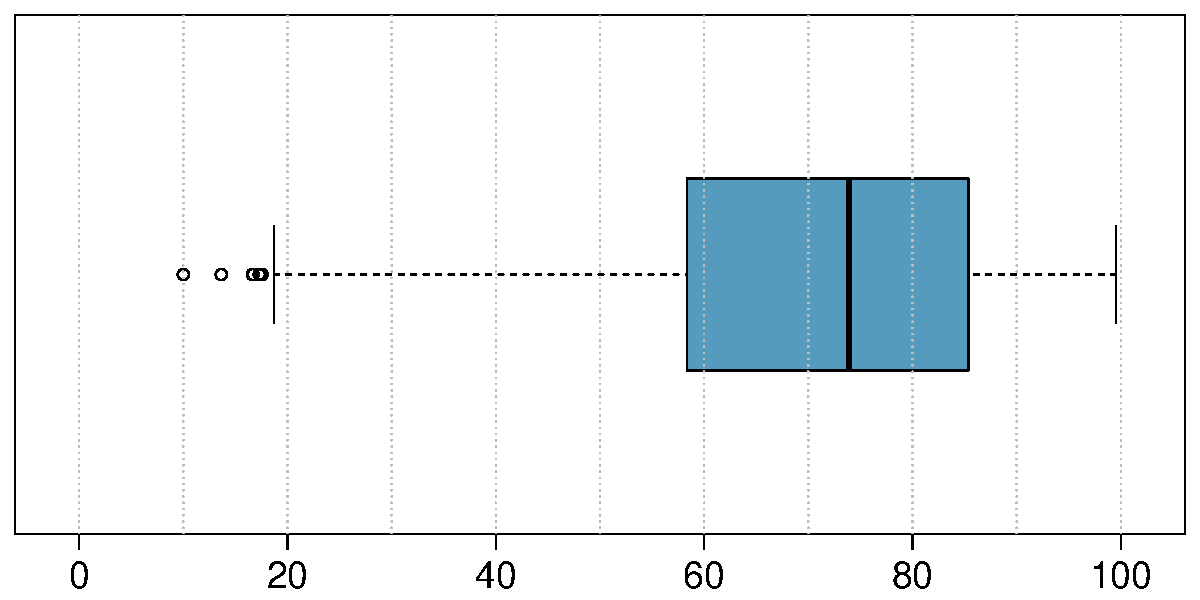
\includegraphics[width=0.7\textwidth]{figures/num_data/boxplot}
\end{center}

\begin{enumerate}[(a)]
\item Fewer observations are above 90 than below 90.
\item \solnMult{Fewer observations are below 60 than above 60.}
\item Fewer observations are below 50 than above 50.
\item The distribution is left skewed.
\end{enumerate}

\end{frame}

%%%%%%%%%%%%%%%%%%%%%%%%%%%%%%%%%%%%

\subsection{Probability}

%%%%%%%%%%%%%%%%%%%%%%%%%%%%%%%%%%%%

\begin{frame}

\clicker{Which of the following is \underline{true}?}

\twocol{0.5}{0.5}{
\begin{enumerate}[(a)]
\item A and B are independent.
\item P(A but not B) = 0.2
\item P(A $|$ B) = 0.06 / 0.14
\item \solnMult{P(A or B) = 0.14 + 0.06 + 0.19}
\item P(neither A nor B) = 1 - 0.06
\end{enumerate}
}
{
\begin{center}
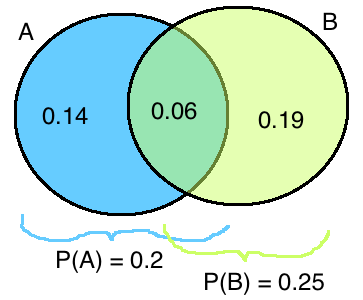
\includegraphics[width=\textwidth]{figures/venn/venn}
\end{center}
}

\end{frame}

%%%%%%%%%%%%%%%%%%%%%%%%%%%%%%%%%%%%

\subsection{Hypothesis testing and confidence intervals}

%%%%%%%%%%%%%%%%%%%%%%%%%%%%%%%%%%%%

\begin{frame}
\frametitle{}

\clicker{We want to conduct the following hypothesis test. Which is the correct distribution/p-value sketch associated with it?
\[H_0: \mu = 100; H_A: \mu \ne 100 \qquad \bar{x} = 95, s = 30, n = 100\]
}

\begin{multicols}{2}
\begin{enumerate}[(a)]
\item 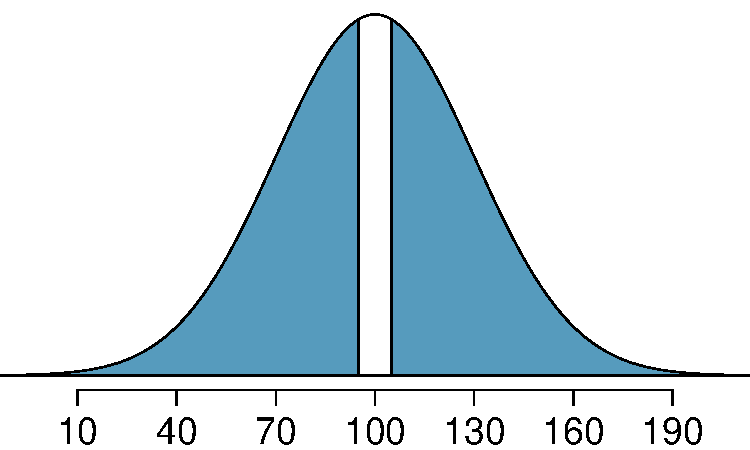
\includegraphics[width=0.35\textwidth]{figures/ht_curves/a}
\item 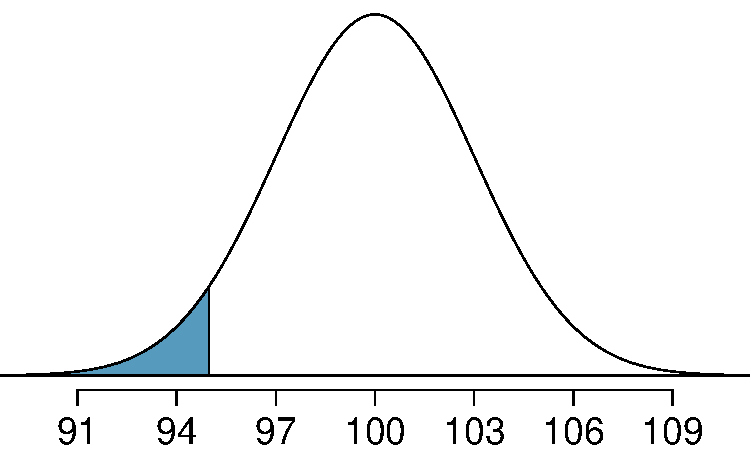
\includegraphics[width=0.35\textwidth]{figures/ht_curves/b}
\item 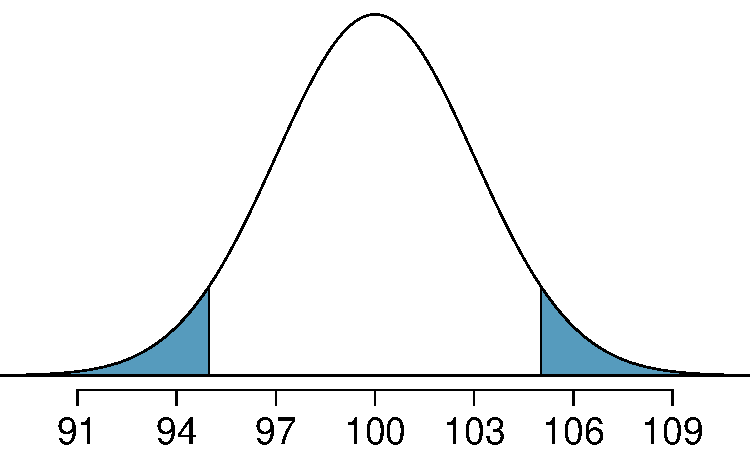
\includegraphics[width=0.35\textwidth]{figures/ht_curves/c}
\item 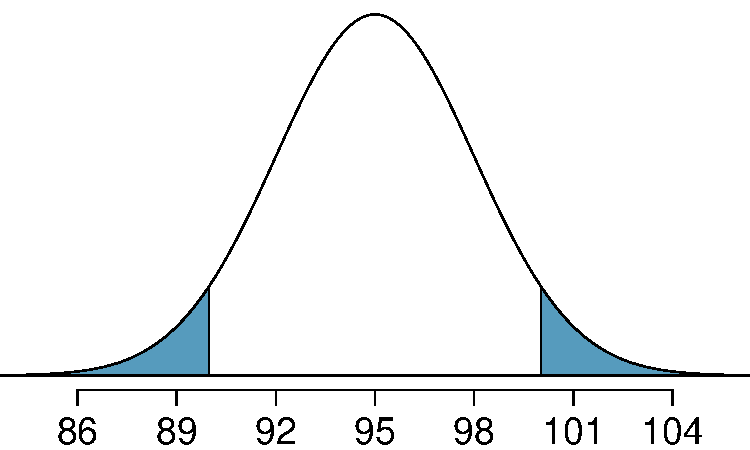
\includegraphics[width=0.35\textwidth]{figures/ht_curves/d}
\end{enumerate}
\end{multicols}

\end{frame}

%%%%%%%%%%%%%%%%%%%%%%%%%%%%%%%%%%%%

\begin{frame}
\frametitle{}

\disc{{\small A random sample of 36 female college-aged dancers was obtained and their heights (in inches) were measured. Provided below are some summary statistics and a histogram of the distribution of these dancers' heights. The average height of all college-aged females is 64.5 inches. Do these data provide convincing evidence that the average height of female college-aged dancers is \emph{lower} from this value?}

\begin{center}
\begin{minipage}[c]{0.3\textwidth}
\begin{center}
\renewcommand\arraystretch{1.5}
\begin{tabular}{l | c }
$n$			& 36 \\
\hline
$mean$		& 63.6 inches \\
\hline
$sd$			& 2.13 inches
\end{tabular}
\end{center}
\end{minipage}
\begin{minipage}[c]{0.6\textwidth}
\begin{center}
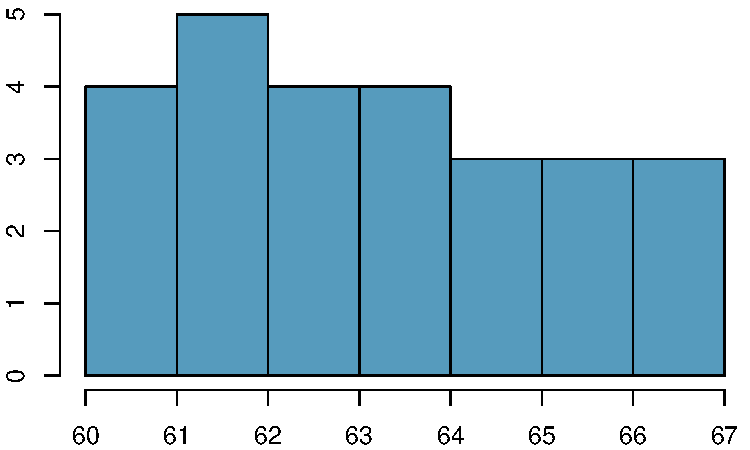
\includegraphics[width=0.5\textwidth]{figures/dancer/dancer}
\end{center}
\end{minipage}
\end{center}
}

\pause

\begin{center}
$H_0: \mu = 64.5$ \\
$H_A: \mu < 64.5$
\end{center}

\vspace{-5mm}


\pause
\[ \bar{x} = 63.6, s = 2.13, n = 36, \alpha = 0.05 \]

\end{frame}

%%%%%%%%%%%%%%%%%%%%%%%%%%%%%%%%%%%%

\begin{frame}

\[ \bar{x} \sim N \left( mean = 64.5, SE = \frac{2.13}{\sqrt{36}} = 0.355 \right) \]
\pause
\[ Z = \frac{63.6 - 64.5}{0.355} = -2.54 \]
\pause
\[ p-value = P(Z < -2.54) = 0.0055 \]

\pause

Since p-value $<$ 0.05, reject $H_0$. The data provide convincing evidence that the average height of female college-aged dancers is lower than 64.5 inches.


\end{frame}

%%%%%%%%%%%%%%%%%%%%%%%%%%%%%%%%%%%%

\begin{frame}

\clicker{Which of the following is the correct interpretation of the p-value?}

\begin{enumerate}[(a)]
\item If in fact the average height of college aged dancers is less than 64.5 inches, the probability of observing a random sample of 36 where the average height is 63.6 inches or lower is 0.0055.
\item \solnMult{If in fact the average height of college aged dancers is 64.5 inches, the probability of observing a random sample of 36 where the average height is 63.6 inches or lower is 0.0055.}
\item If in fact the average height of college aged dancers is 64.5 inches, the probability of observing a random sample of 36 where the average height is 63.6 inches is 0.0055.
\item The probability that the average height of college aged dancers is 64.5 inches is 0.0055.
\end{enumerate}

\end{frame}

%%%%%%%%%%%%%%%%%%%%%%%%%%%%%%%%%%%%

\begin{frame}

\clicker{What is the equivalent confidence level for this one-sided hypothesis test with $\alpha = 0.05$?}

\begin{enumerate}[(a)]
\item 80\%
\item \solnMult{90\%}
\item 95\%
\item 99.7\%
\item 97.5\%
\end{enumerate}

\end{frame}

%%%%%%%%%%%%%%%%%%%%%%%%%%%%%%%%%%%%

\begin{frame}

\clicker{If we were to calculate a 95\% confidence interval for the average height of college-aged dancers, would this interval include the null value (64.5 inches)?}

\begin{enumerate}[(a)]
\item Yes
\item No
\item \solnMult{Cannot tell without calculating the interval}
\end{enumerate}

\end{frame}

%%%%%%%%%%%%%%%%%%%%%%%%%%%%%%%%%%%%

\subsection{Randomization testing}

%%%%%%%%%%%%%%%%%%%%%%%%%%%%%%%%%%%%

\begin{frame}

{\small CPR is a procedure commonly used on individuals suffering a heart attack when other emergency resources are not available. The chest compressions involved with this procedure can also cause internal injuries. Blood thinners that are often given to help release a clot that is causing the heart attack may also negatively affect such internal injuries. An experiment was designed to evaluate if blood thinners have an impact on survival after a heart attack. Patients were randomly divided into a treatment group (received a blood thinner) or the control group (no blood thinner). The outcome variable of interest was whether the patients survived for at least 24 hours.}

\end{frame}

%%%%%%%%%%%%%%%%%%%%%%%%%%%%%%%%%%%%

\begin{frame}

\disc{Form hypotheses for this study in plain and statistical language. Let $p_c$ represent the true survival proportion in the control group and $p_t$ represent the survival proportion for the treatment group.}

\begin{itemize}
\item[$H_0$:] Blood thinners do not have an overall survival effect, i.e. the survival proportions are the same in each group. $p_t - p_c = 0$.
\item[$H_A$:] Blood thinners do have an impact on survival. $p_t - p_c \neq 0$.
\end{itemize}

\end{frame}

%%%%%%%%%%%%%%%%%%%%%%%%%%%%%%%%%%%%

\begin{frame}

\clicker{Given these hypotheses, what is the sample statistic?
\[ H_0: p_t - p_c = 0 \qquad H_A: p_t - p_c \neq 0 \]
}

\begin{center}
\begin{tabular}{lccccc}
\hline
			&& Survived 	& Died 	&& Total \\
\hline
Control		&& 11		& 39		&& 50 \\
Treatment		&& 14		& 26		&& 40 \\
\hline
Total			&& 25		& 65		&& 90 \\
\hline
\end{tabular}
\end{center}

\begin{enumerate}[(a)]
\item (11 / 25) - (39 / 65) = -0.16
\item \solnMult{(14 / 40) - (11 / 50) = 0.13}
\item (14 / 90) - (11 / 90) = 0.033
\item (40 / 90) - (50 / 90) = -0.111
\end{enumerate}

\end{frame}

%%%%%%%%%%%%%%%%%%%%%%%%%%%%%%%%%%%%

\begin{frame}

\clicker{{\small A randomization test was conducted to evaluate these hypotheses. Based on the randomization distribution below, what is the conclusion?}}

\begin{center}
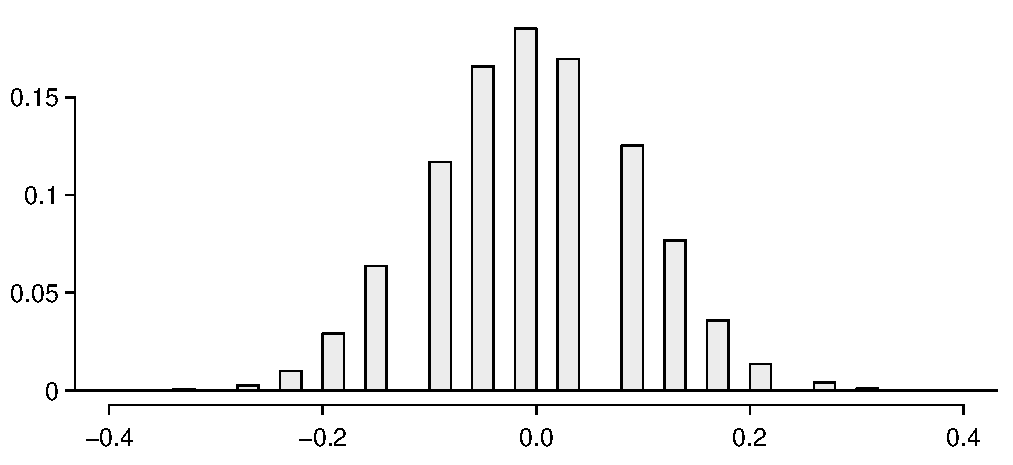
\includegraphics[width=0.57\textwidth]{figures/cpr/cpr_rand_dist}
\end{center}

{\small
These data 
\begin{enumerate}[(a)]
\item provide convincing evidence that blood thinners 
\item provide convincing evidence that blood thinners do not
\item \solnMult{do not provide convincing evidence that blood thinners}
\item do not provide convincing evidence that blood thinners do not
\end{enumerate}
have an impact on survival.
}

\end{frame}

%%%%%%%%%%%%%%%%%%%%%%%%%%%%%%%%%%%%

\subsection{Binomial distribution}

%%%%%%%%%%%%%%%%%%%%%%%%%%%%%%%%%%%%

\begin{frame}

\clicker{Which of the following probabilities should be calculated using the Binomial distribution?}

Probability that
\begin{enumerate}[(a)]
\item \solnMult{a basketball player misses 3 times in 5 shots} \soln{\only<2>{{\red{$\rightarrow$ k successes in n trials}}}}
\item train arrives on the time on the third day for the first time
\item height of a randomly chosen 5 year old is greater than 4 feet
\item a randomly chosen individual likes chocolate ice cream best
\end{enumerate}

\end{frame}

%%%%%%%%%%%%%%%%%%%%%%%%%%%%%%%%%%%%

\begin{frame}
\frametitle{Why Binomial?}

\disc{Suppose the probability of a miss for this basketball player is 0.40. What is the probability that she misses 3 times in 5 shots?}

\pause

\begin{itemize}

\item One possible scenario is that she misses the first three shots, and makes the last two. The probability of this scenario is:
\[ 0.4^3 \times 0.6^2 \approx 0.023 \]

\pause

\item But this isn't the only possible scenario:
\vspace{-0.25cm}
\begin{changemargin}{-1.5cm}{0cm} 
\begin{multicols}{5}
\begin{enumerate}[1.]
\item \red{M}\red{M}\red{M}HH
\item \red{M}\red{M}H\red{M}H
\item \red{M}H\red{M}\red{M}H
\item H\red{M}\red{M}\red{M}H
\item H\red{M}\red{M}H\red{M}
\item H\red{M}H\red{M}\red{M}
\item HH\red{M}\red{M}\red{M}
\item \red{M}H\red{M}H\red{M}
\item \red{M}HH\red{M}\red{M}
\item \red{M}\red{M}HH\red{M}
\end{enumerate}
\end{multicols}
\end{changemargin}

\pause

\item Each one of these scenarios has 3 \red{M}s and 2 Hs, therefore the probability of each scenario is $0.023$.

\pause

\item Then, the total probability is $10 \times 0.023 = 0.23$.

\end{itemize}

\end{frame}

%%%%%%%%%%%%%%%%%%%%%%%%%%%%%%%%%%%%

\begin{frame}
\frametitle{... concisely}

\disc{Suppose the probability of a miss for this basketball player is 0.40. What is the probability that she misses 3 times in 5 shots?}

\pause

\begin{eqnarray*} 
{5 \choose 3} \times 0.4^3 \times 0.6^2 &=& \frac{5!}{3! \times 2!} \times 0.4^3 \times 0.6^2 \\
\pause
&=& 10 \times 0.023 \\
\pause
&=& 0.23
\end{eqnarray*}

\end{frame}

%%%%%%%%%%%%%%%%%%%%%%%%%%%%%%%%%%%%

\begin{frame}
\frametitle{}

\clicker{Which of the following highlights the correct outcomes for ``at most 3 misses in 5 shots"?}

\begin{enumerate}[(a)]
\item \{\orange{0, 1, 2}, 3, 4, 5\} 
\item \solnMult{\{\orange{0, 1, 2, 3}, 4, 5\}}
\item  \{0, 1, 2, \orange{3, 4, 5}\}
\item \{0, 1, 2, \orange{3}, 4, 5\}
\item \{0, 1, 2, \orange{3, 4}, 5\}
\end{enumerate}

\end{frame}

%%%%%%%%%%%%%%%%%%%%%%%%%%%%%%%%%%%%

\begin{frame}
\frametitle{}

\clicker{Which of the following is the correct calculation for ``P(at most 3 misses in 5 shots)"? \\
{\small Note: P(k) means P(k misses in 5 shots), calculated using the binomial formula.}
}

\begin{enumerate}[(a)]
\item P(0) + P(1) + P(2)
\item P(3) + P(4) + P(5)
\item 1 - P(0)
\item 1 - [ P(0) + P(1) + P(2)]
\item \solnMult{1 - [ P(4) + P(5) ]}
\end{enumerate}

\end{frame}

%%%%%%%%%%%%%%%%%%%%%%%%%%%%%%%%%%%%

\subsection{Conditional probability}

%%%%%%%%%%%%%%%%%%%%%%%%%%%%%%%%%%%%

\begin{frame}
\frametitle{Testing for AIDS -- with counts}

\disc{Suppose that the proportion of people infected with AIDS in a large population is 0.01. If AIDS is present, a certain medical test is positive with probability 0.997 (called the sensitivity of the test). If AIDS is not present, the test is negative with probability 0.985 (called the specificity of the test). If a person tests positive, what is the probability that they have AIDS?}

\pause

\begin{itemize}

\item Let's assume there are 1 million individuals in this population.

\pause

\item How many are expected to have AIDS, and how many are not expected to have AIDS?
\pause
\begin{itemize}
\item Have AIDS: $1,000,000 \times 0.01 = 10,000$
\pause
\item Don't have AIDS: $1,000,000 \times 0.99 = 990,000$
\end{itemize}

\end{itemize}

\ct{From \webURL{http://www.pitt.edu/~nancyp/stat-1000-s07/week6.pdf}.}

\end{frame}

%%%%%%%%%%%%%%%%%%%%%%%%%%%%%%%%%%%%

\begin{frame}
\frametitle{Testing for AIDS -- with counts (cont.)}

\clicker{How many of the people with AIDS would we expect to test positive?}

\begin{enumerate}[(a)]
\item 30
\item 9,850
\item \solnMult{9,970} \soln{\only<2>{\red{$\rightarrow 10,000 \times 0.997 = 9970$}}}
\item 987,030
\item 997,000
\end{enumerate}

\end{frame}

%%%%%%%%%%%%%%%%%%%%%%%%%%%%%%%%%%%%

\begin{frame}
\frametitle{Testing for AIDS -- with counts (cont.)}

\begin{changemargin}{-0.75cm}{-0.75cm} 

% Set the overall layout of the tree
\tikzstyle{level 1}=[level distance=3cm, sibling distance=3.5cm]
\tikzstyle{level 2}=[level distance=3cm, sibling distance=2cm]

% Define styles for bags and leafs
\tikzstyle{bag} = [text width=4em, text centered]
\tikzstyle{end} = [circle, minimum width=3pt,fill, inner sep=0pt]

\only<1| handout:0>{
\begin{tikzpicture}[grow=right, sloped]
\node[bag] {\green{1,000,000}}
    child {
        node[bag] {no AIDS: \green{990,000}}        
            edge from parent 
            node[above] {}
            node[below]  {$0.99$}
    }
    child {
        node[bag] {AIDS: \green{10,000}}        
        edge from parent         
            node[above] {$$}
            node[below]  {$0.01$}
    };
\end{tikzpicture}
}

\only<2|handout:0>{
\begin{tikzpicture}[grow=right, sloped]
\node[bag] {\green{1,000,000}}
    child {
        node[bag] {no AIDS: \green{990,000}}        
            edge from parent 
            node[above] {}
            node[below]  {$0.99$}
    }
    child {
        node[bag] {AIDS: \green{10,000}}        
        child {
                node[end, label=right:
                    {10,000 $\times$ 0.003 = \green{30}}] {}
                edge from parent
                node[above] {$-$}
                node[below]  {$0.003$}
            }
            child {
                node[end, label=right:
                    {10,000 $\times$ 0.997 = \green{9,970}}] {}
                edge from parent
                node[above] {$+$}
                node[below]  {$0.997$}
            }
        edge from parent         
            node[above] {$$}
            node[below]  {$0.01$}
    };
\end{tikzpicture}
}

\only<3->{
\begin{tikzpicture}[grow=right, sloped]
\node[bag] {\green{1,000,000}}
    child {
        node[bag] {no AIDS: \green{990,000}}        
            child {
                node[end, label=right:
                    {990,000 $\times$ 0.985 = \green{975,150}}] {}
                edge from parent
                node[above] {$-$}
                node[below]  {$0.985$}
            }
            child {
                node[end, label=right:
                    {990,000 $\times$ 0.015 = \green{14,850}}] {}
                edge from parent
                node[above] {$+$}
                node[below]  {$0.015$}
            }
            edge from parent 
            node[above] {}
            node[below]  {$0.99$}
    }
    child {
        node[bag] {AIDS: \green{10,000}}        
        child {
                node[end, label=right:
                    {10,000 $\times$ 0.003 = \green{30}}] {}
                edge from parent
                node[above] {$-$}
                node[below]  {$0.003$}
            }
            child {
                node[end, label=right:
                    {10,000 $\times$ 0.997 = \green{9,970}}] {}
                edge from parent
                node[above] {$+$}
                node[below]  {$0.997$}
            }
        edge from parent         
            node[above] {$$}
            node[below]  {$0.01$}
    };
\end{tikzpicture}
}

\end{changemargin}

\only<4->{
\[ P(AIDS | +) = \frac{9,970}{9,970 + 14,850} \approx 0.40 \]
}

\end{frame}

%%%%%%%%%%%%%%%%%%%%%%%%%%%%%%%%%%%%

\begin{frame}
\frametitle{Testing for AIDS -- with probabilities}

\begin{changemargin}{-1cm}{-1cm} 

% Set the overall layout of the tree
\tikzstyle{level 1}=[level distance=3cm, sibling distance=3.5cm]
\tikzstyle{level 2}=[level distance=3cm, sibling distance=2cm]

% Define styles for bags and leafs
\tikzstyle{bag} = [text width=4em, text centered]
\tikzstyle{end} = [circle, minimum width=3pt,fill, inner sep=0pt]

% The sloped option gives rotated edge labels. Personally
% I find sloped labels a bit difficult to read. Remove the sloped options
% to get horizontal labels. 
\begin{tikzpicture}[grow=right, sloped]
\node[bag] {}
    child {
        node[bag] {no AIDS}        
            child {
                node[end, label=right:
                    {$P(no~AIDS~\&~-)=0.99 \times 0.985$}] {}
                edge from parent
                node[above] {$-$}
                node[below]  {$0.985$}
            }
            child {
                node[end, label=right:
                    {$P(no~AIDS~\&~+)=0.99 \times 0.015$}] {}
                edge from parent
                node[above] {$+$}
                node[below]  {$0.015$}
            }
            edge from parent 
            node[above] {}
            node[below]  {$0.99$}
    }
    child {
        node[bag] {AIDS}        
        child {
                node[end, label=right:
                    {$P(AIDS~\&~-)=0.01 \times 0.003$}] {}
                edge from parent
                node[above] {$-$}
                node[below]  {$0.003$}
            }
            child {
                node[end, label=right:
                    {$P(AIDS~\&~+)=0.01 \times 0.997$}] {}
                edge from parent
                node[above] {$+$}
                node[below]  {$0.997$}
            }
        edge from parent         
            node[above] {$$}
            node[below]  {$0.01$}
    };
\end{tikzpicture}

\end{changemargin}

\pause

\[ P(AIDS | +) = \frac{0.01 \times 0.997}{0.01 \times 0.997 + 0.99 \times 0.015} \approx 0.40 \]

\end{frame}

%%%%%%%%%%%%%%%%%%%%%%%%%%%%%%%%%%%%

\begin{frame}
\frametitle{Testing for AIDS --  in a Bayesian framework}

\begin{itemize}

\item In the first stage of testing:
\begin{itemize}
\item Prior: P(AIDS) \\ 
= P(person has AIDS before we collect any data on them) = 0.01
\item Posterior: P(AIDS $|$ test +) \\
= P(person has AIDS \hl{given} that they tested positive) = 0.40
\end{itemize}
\item In the second stage of testing:
\begin{itemize}
\item Prior = Posterior from the previous test = 0.40
\end{itemize}

\end{itemize}

\vfill

\disc{If the person tests positive for AIDS in the first test, will the prior probability be higher or lower than 1\% (prior in the first test)? Why?}


\soln{\pause{Higher, we're more likely to think that they have AIDS, compared to an average person from this population, since they tested positive once.}}


\end{frame}

%%%%%%%%%%%%%%%%%%%%%%%%%%%%%%%%%%%%

\end{document}

\begin{frame}

\disc{{\small A housing survey was conducted to determine the price of a typical home in Topanga, CA. The mean price of a house was roughly \$1.3 million with a standard deviation of \$300,000. There were no houses listed below \$600,000 but a few houses above \$3 million.}}

\clicker{Can we estimate the probability that a randomly chosen house in Topanga costs more than \$1.4 million using the normal distribution?}

\begin{enumerate}[(a)]
\item yes
\item \solnMult{no}
\end{enumerate}

\end{frame}

%%%%%%%%%%%%%%%%%%%%%%%%%%%%%%%%%%%

\begin{frame}

\disc{{\small A housing survey was conducted to determine the price of a typical home in Topanga, CA. The mean price of a house was roughly \$1.3 million with a standard deviation of \$300,000. There were no houses listed below \$600,000 but a few houses above \$3 million.}}

\clicker{Can we estimate the probability that the mean of 60 randomly chosen houses in Topanga is more than \$1.4 million?}

\begin{enumerate}[(a)]
\item \solnMult{yes}
\item no
\end{enumerate}

\end{frame}

%%%%%%%%%%%%%%%%%%%%%%%%%%%%%%%%%%%%

\begin{frame}

\disc{{\small A housing survey was conducted to determine the price of a typical home in Topanga, CA. The mean price of a house was roughly \$1.3 million with a standard deviation of \$300,000. There were no houses listed below \$600,000 but a few houses above \$3 million.}}

\disc{{\small What is the probability that the mean of 60 randomly chosen houses in Topanga is more than \$1.4 million?}}

\pause

In order to calculate $P(\bar{X} > 1.4~mil)$, we need to first determine the distribution of $\bar{X}$. According to the CLT,

\pause

\[ \bar{X} \pause \sim N \pause \left( mean = 1.3, \pause SE = \frac{0.3}{\sqrt{60}} = 0.0387 \right) \]

\pause

\begin{eqnarray*}
P(\bar{X} > 1.4 ) &=& P\left(Z > \frac{1.4 - 1.3}{0.0387}\right) \\
\pause
&=& P(Z > 2.58) \\
\pause
&=& 1 - 0.9951 \pause =  0.0049
\end{eqnarray*}

\end{frame}

%%%%%%%%%%%%%%%%%%%%%%%%%%%%%%%%%%%%


\end{document}